\documentclass[border=12pt,tikz]{standalone}
\usetikzlibrary{backgrounds, positioning}
\usepackage[T1]{fontenc}
\usepackage[scaled=0.98]{helvet}

\definecolor{colE}{RGB}{160,82,20}   % espresso: brown
\definecolor{colM}{RGB}{70,110,190}  % milk: blue
\definecolor{colC}{RGB}{0,150,160}   % cold: cyan

\begin{document}
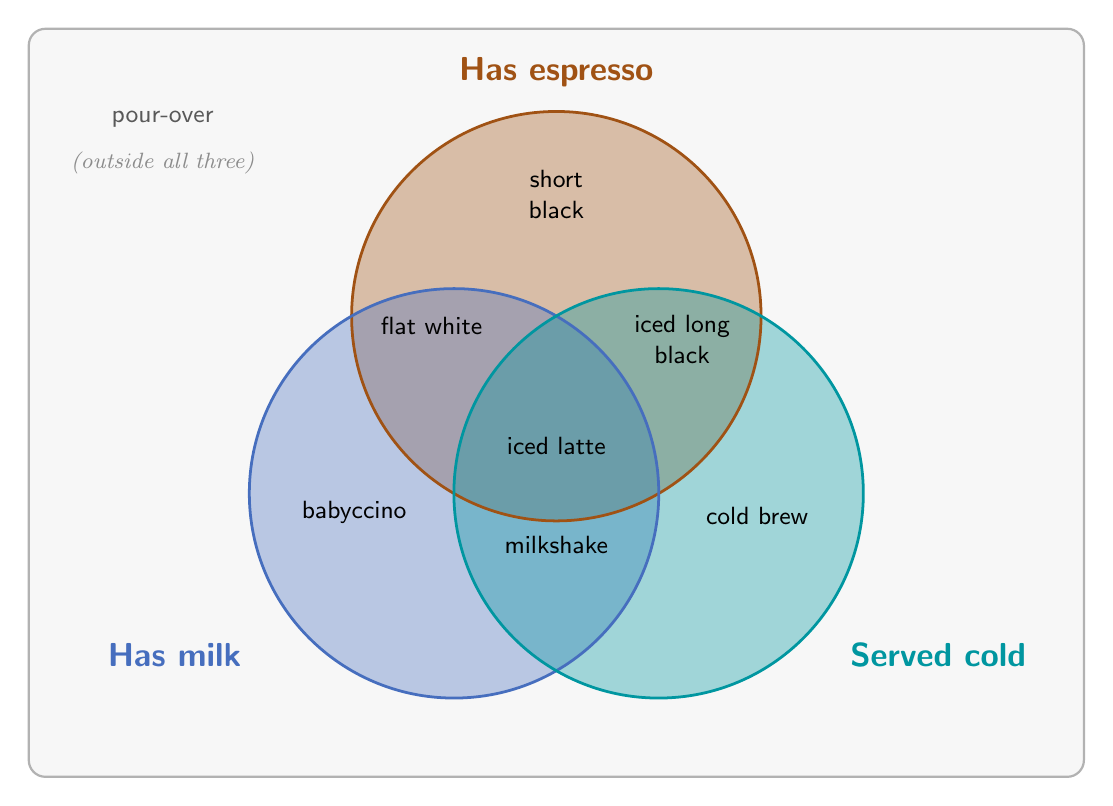
\begin{tikzpicture}[
    font=\sffamily,
    drink/.style={text width=2.4cm, align=center, inner sep=1pt, font=\small\sffamily},
    setlabel/.style={font=\large\bfseries\sffamily, inner sep=2pt},
  ]

  \def\R{2.6cm}   % circle radius
  \def\d{1.5cm}   % distance of each centre from the middle

  \coordinate (E) at (90:\d);    %  Has espresso
  \coordinate (M) at (210:\d);   %  Has milk
  \coordinate (C) at (330:\d);   %  Served cold

  % ---- the universe (everything that is not in any circle lives here) ---
  \begin{scope}[on background layer]
    \fill[black!3, rounded corners=6pt] (-6.7,-4.35) rectangle (6.7,5.15);
  \end{scope}
  \draw[black!30, line width=0.8pt, rounded corners=6pt] (-6.7,-4.35) rectangle (6.7,5.15);

  % ---- filled circles (behind the labels) -------------------------------
  \begin{scope}[on background layer]
    \fill[colE, fill opacity=0.35] (E) circle (\R);
    \fill[colM, fill opacity=0.35] (M) circle (\R);
    \fill[colC, fill opacity=0.35] (C) circle (\R);
  \end{scope}
  \draw[colE, line width=1pt] (E) circle (\R);
  \draw[colM, line width=1pt] (M) circle (\R);
  \draw[colC, line width=1pt] (C) circle (\R);

  % ---- set labels -------------------------------------------------------
  \node[setlabel, colE] at (0,4.6)     {Has espresso};
  \node[setlabel, colM] at (210:5.6cm) {Has milk};
  \node[setlabel, colC] at (330:5.6cm) {Served cold};

  % ---- the drinks -------------------------------------------------------
  % espresso only (hot shot, no milk)
  \node[drink] at (90:3.05cm)            {short\\ black};
  % milk only (steamed milk, no coffee)
  \node[drink] at (201:2.75cm)           {babyccino};
  % cold only (brewed black, served over ice)
  \node[drink] at (338:2.75cm)           {cold brew};
  % espresso + milk, served hot
  \node[drink] at (139:2.10cm)           {flat white};
  % espresso + cold, no milk
  \node[drink, text width=1.9cm] at (37:2.0cm) {iced long\\ black};
  % milk + cold, no espresso
  \node[drink] at (270:1.40cm)           {milkshake};
  % all three
  \node[drink] at (0,-0.15)              {iced latte};
  % none of the three: hot, brewed (not espresso), no milk
  \node[drink, text=black!65] at (-5.0,4.0) {pour-over};
  \node[drink, font=\footnotesize\itshape, text=black!45, text width=3.2cm]
       at (-5.0,3.45) {(outside all three)};

\end{tikzpicture}
\end{document}
